%!TEX root = ../Thesis.tex

\section{Methods for variance reduction}
This section explores the effects of different variance reduction methods. If nothing else is noted, the training details are as described in \autoref{sec: Experimental work: Effects of common model and algorithm augmentations}.

\subsection{Gradient momentum}\label{sec: Experimental work: Effect of momentum}
Due to the potentially high variance of the \gls{VO} gradient, the use of momentum (see \autoref{sec: Neural networks training: Optimization: SGD with momentum}) can have a positive effect on the convergence speed and training time of \gls{VO}. Three levels of momentum were run for thirty random seeds each. The momentums were $0$, $0.1$ and $0.9$. The results can be seen in \autoref{fig: Theory: E030-MOM-S-analysis}. 
A small benefit can be noted from using a momentum of $0.1$ while using $0.9$ has a large impact on the convergence speed.
It is evident that the \gls{VO} gradient benefits from including momentum.

A momentum of $0.99$ was also included in this experiment but resulted in the algorithm not converging. Instead, the training achieved losses of about $0.6$, oscillating up and down presumably due to the gradient being too dependent on past values to adequately adapt to the loss surface. It is plausible that an optimal value of the momentum for this problem resides somewhere between $0.99$ and $0.1$ but no attempt will be made at finding this value.

When adapting the variance, the effect of momentum on the variance was also examined and found to occasionally be detrimental, especially in the \gls{RL} setting. At times, the gradient associated with the variance would spike at a single iteration, preceded and followed by much smaller gradients. Momentum would then continue to increase the variance for many iterations following the spike resulting in a large variance giving detrimentally large perturbations. Lowering the variance learning rate results in the variance practically not adapting during training. Using dampened momentum aids in suppressing these spikes and is discussed further in \autoref{sec: Experimental work: Effect of adapting the variance}. Alternatively, not using momentum on the variance gradient gives little weight to these spikes and the trend of decreasing variance persists through training as wanted.

\begin{figure}[tbp!]
    \begin{subfigure}[b]{0.49\textwidth}
        \centering
        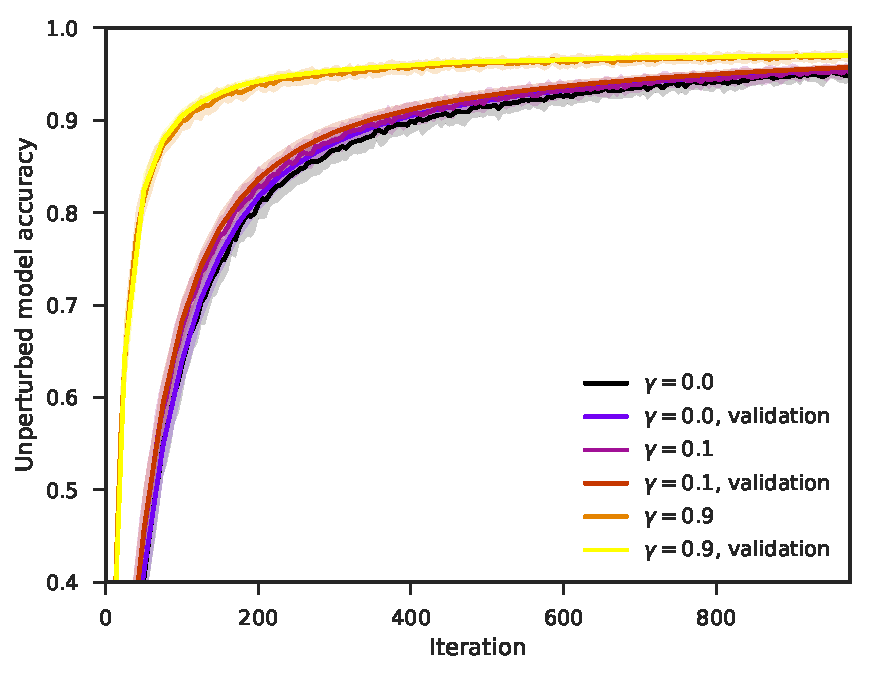
\includegraphics[height=5.8cm]{graphics/E030-MOM-S-analysis/accuracy_unp-all-series-mean-sd.pdf}
        \caption{}
        \label{fig: Theory: E030-MOM-S-analysis/accuracy_unp-all-series-mean-sd}
    \end{subfigure}
    \hfill
    \begin{subfigure}[b]{0.49\textwidth}
        \centering
        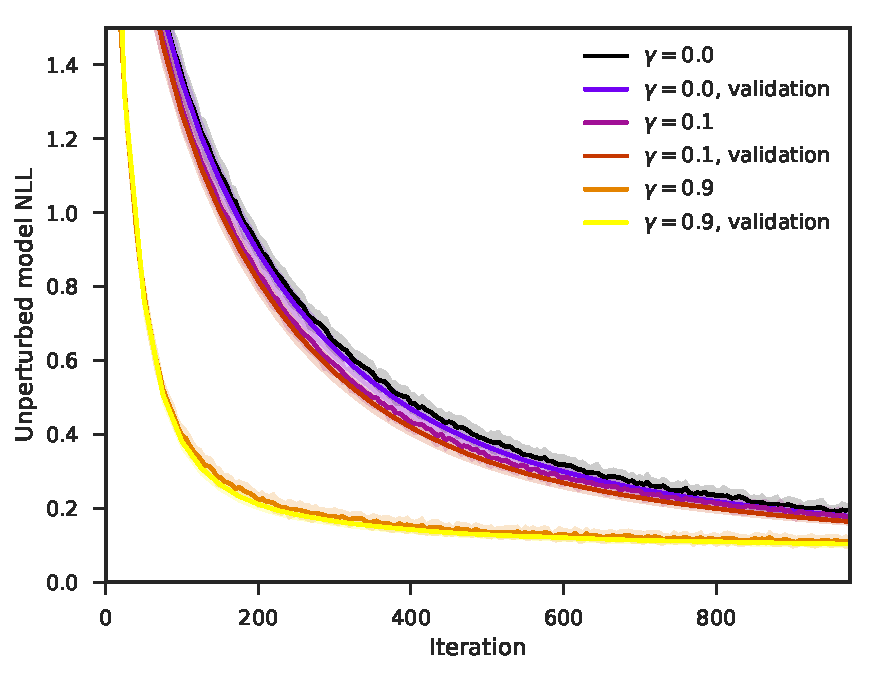
\includegraphics[height=5.8cm]{graphics/E030-MOM-S-analysis/return_unp-all-series-mean-sd.pdf}
        \caption{}
        \label{fig: Theory: E030-MOM-S-analysis/return_unp-all-series-mean-sd}
    \end{subfigure}
    \caption{
        Results of experiments using \gls{SGD} with momentum on the \gls{VO} gradient for the unperturbed model run on \gls{MNIST}.
        \subref{fig: Theory: E030-MOM-S-analysis/accuracy_unp-all-series-mean-sd} Training and validation set classification accuracy.
        \subref{fig: Theory: E030-MOM-S-analysis/return_unp-all-series-mean-sd} Training and validation set \gls{NLL} loss.
        Gradient momentum is effective at reducing the gradient variance and results in faster convergence.
    }
    \label{fig: Theory: E030-MOM-S-analysis}
\end{figure}


\subsection{Antithetic sampling}\label{sec: Experimental work: Antithetic sampling}
In this section, the improvement by using antithetic sampling is experimentally validated. The \gls{MNIST} network was trained using 100 perturbations with antithetic sampling (50 unique, 50 mirrored), 100 perturbations without antithetic sampling and 50 perturbations without antithetic sampling. 

The runs using 100 perturbations with antithetic sampling compares to the runs using 100 perturbations without antithetic sampling in the way that both estimate the gradient from 100 perturbations. From this comparison it can be assessed whether the antithetic samples carry more information than the regular uninformed samples.

The grounds for comparison of runs using 50 perturbations without and 100 perturbations with antithetic sampling is that both of these versions perturb an 50-dimensional subspace of the network parameter space at every iteration of \glsfirst{VO}.
Additionally, the computational complexity of sampling is half as high when using antithetic sampling.
Obviously, the time complexity of the sampling operation is negligible compared to the fitness evaluation so comparison in this basis is not entirely fair.

The results are shown in \autoref{fig: Theory: E022-AS-analysis}. It is evident that using antithetic sampling results in a significant improvement when comparing to both runs with 50 and 100 perturbations. As opposed to the effect seen when including batch normalization, the loss curves initially rise with approximately the same slope but do not asymptote the same value. Thus, the benefit from using antithetic sampling is not faster training but rather the location of a better local minimum and thus better final performance. This is almost certainly due to a reduction in the gradient estimate variance. 

\begin{figure}[tbp!]
    \begin{subfigure}[b]{0.49\textwidth}
        \centering
        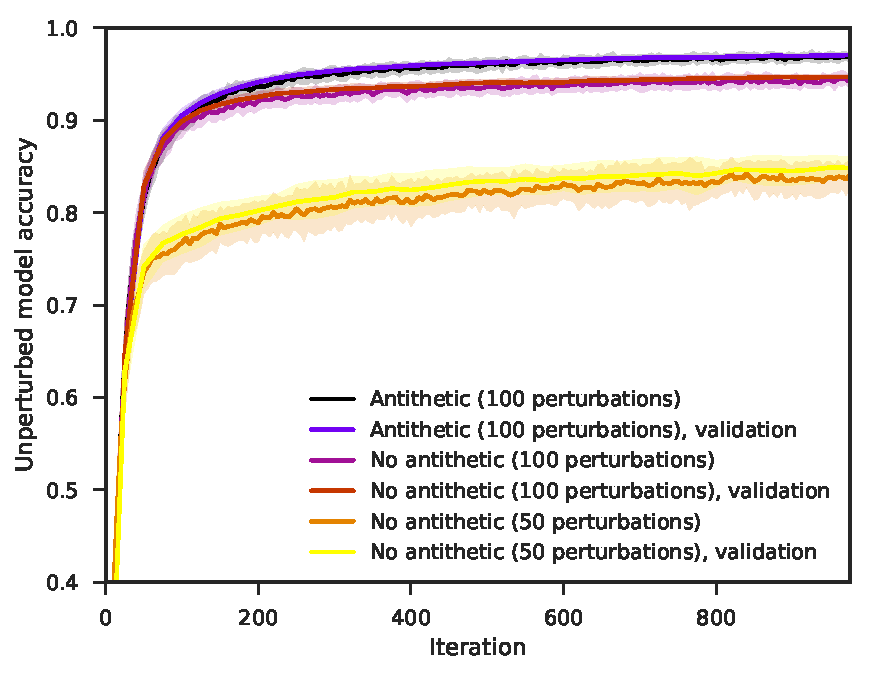
\includegraphics[height=5.8cm]{graphics/E022-AS-analysis/accuracy_unp-all-series-mean-sd.pdf}
        \caption{}
        \label{fig: Theory: E022-AS-analysis/accuracy_unp-all-series-mean-sd}
    \end{subfigure}
    \hfill
    \begin{subfigure}[b]{0.49\textwidth}
        \centering
        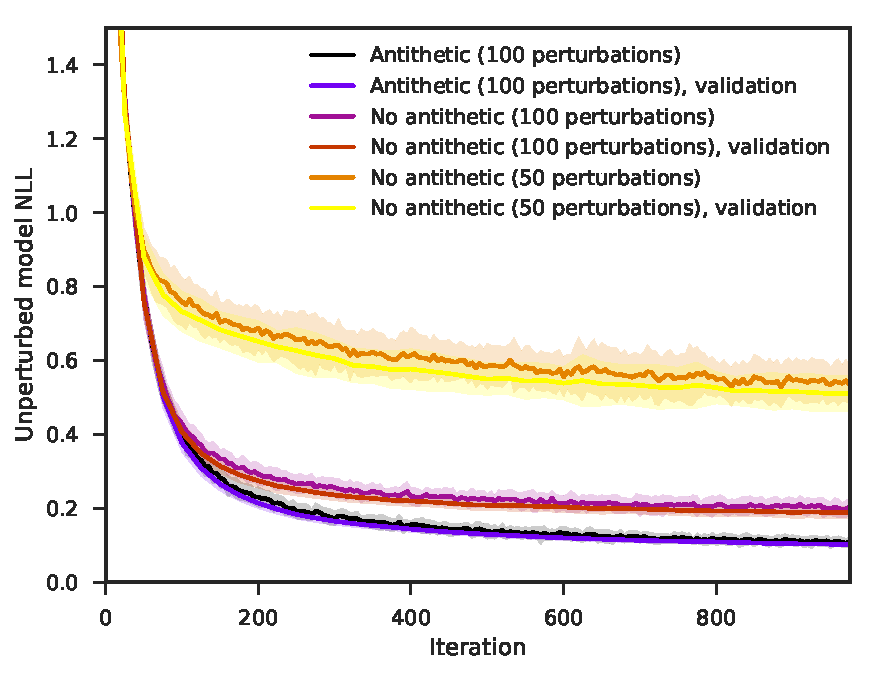
\includegraphics[height=5.8cm]{graphics/E022-AS-analysis/return_unp-all-series-mean-sd.pdf}
        \caption{}
        \label{fig: Theory: E022-AS-analysis/return_unp-all-series-mean-sd}
    \end{subfigure}
    \caption{
        Results of experiments with antithetic sampling for the unperturbed model.
        \subref{fig: Theory: E022-AS-analysis/accuracy_unp-all-series-mean-sd} Training and validation set classification accuracy.
        \subref{fig: Theory: E022-AS-analysis/return_unp-all-series-mean-sd} Training and validation set \gls{NLL} loss.
    }
    \label{fig: Theory: E022-AS-analysis}
\end{figure}

\subsection{Importance mixing}
This section presents results of using importance mixing. This comparison is made in spite of the importance weight collapse and the numerical problems associated with it. In practice some weights become infinite which leads to some reuse of some perturbations. 

\autoref{fig: Theory: E025-IS-analysis} compares a run with importance mixing $(\alpha=0.01)$ and a run without $(\alpha=1.0)$. The \gls{NLL} when using importance mixing is slightly higher than when not. This observation is present in the resulting classification accuracy as well. This detrimental effect must be concluded to stem from the collapse of the importance weights as previously discussed.

\begin{figure}[tbp!]
    \begin{subfigure}[b]{0.49\textwidth}
        \centering
        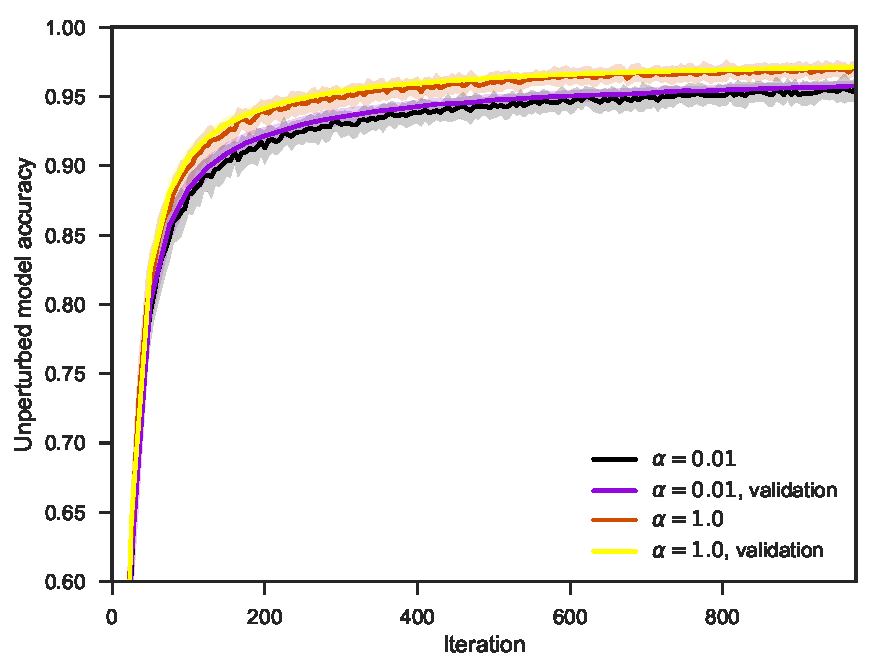
\includegraphics[height=5.8cm]{graphics/E025-IS-analysis/accuracy_unp-all-series-mean-sd.pdf}
        \caption{}
        \label{fig: Theory: E025-IS-analysis/accuracy_unp-all-series-mean-sd}
    \end{subfigure}
    \hfill
    \begin{subfigure}[b]{0.49\textwidth}
        \centering
        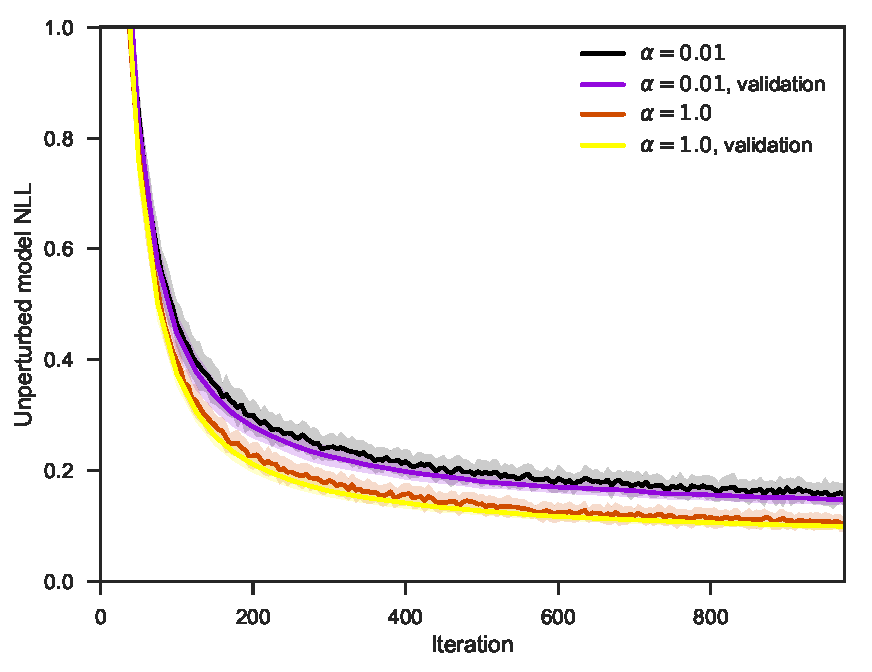
\includegraphics[height=5.8cm]{graphics/E025-IS-analysis/return_unp-all-series-mean-sd.pdf}
        \caption{}
        \label{fig: Theory: E025-IS-analysis/return_unp-all-series-mean-sd}
    \end{subfigure}
    \caption{
        Results of experiments with importance mixing for the unperturbed model.
        \subref{fig: Theory: E025-IS-analysis/accuracy_unp-all-series-mean-sd} Training and validation set classification accuracy.
        \subref{fig: Theory: E025-IS-analysis/return_unp-all-series-mean-sd} Training and validation set \gls{NLL} loss.
    }
    \label{fig: Theory: E025-IS-analysis}
\end{figure}

For comparison, \autoref{fig: Theory: E026-IS-analysis} presents results runs where importance mixing has been replaced by random reuse of perturbations. In the runs with importance mixing, about 10 of the 100 perturbations where effectively reused at each iteration. Therefore, the experiment with random reuse reused 10 perturbations randomly at each iteration. It can be observed that the effect of randomly reusing perturbations is smaller than that of importance mixing, although it remains detrimental compared to reusing no perturbations.

\begin{figure}[tbp!]
    \begin{subfigure}[b]{0.49\textwidth}
        \centering
        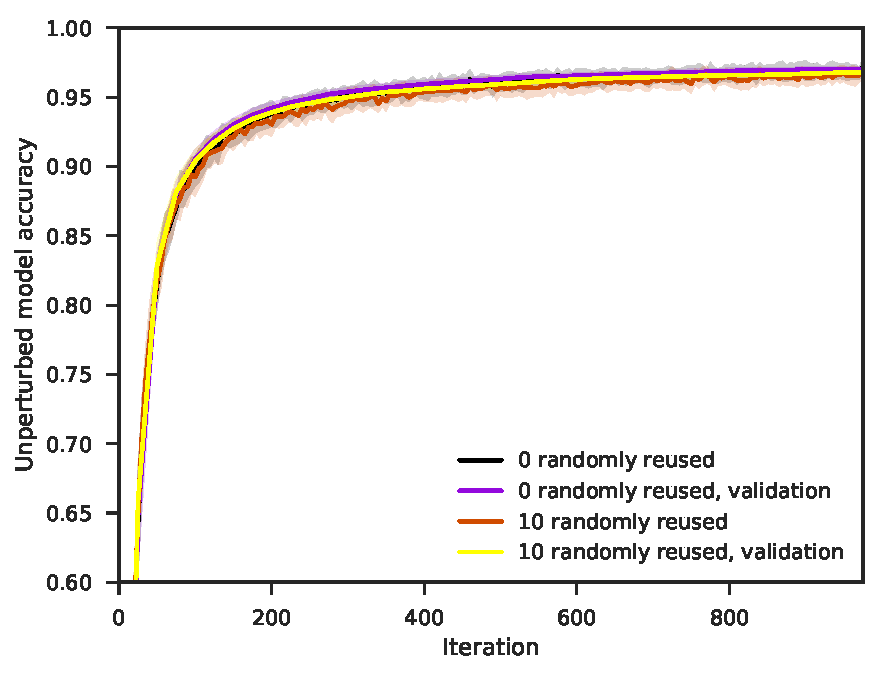
\includegraphics[height=5.8cm]{graphics/E026-IS-analysis/accuracy_unp-all-series-mean-sd.pdf}
        \caption{}
        \label{fig: Theory: E026-IS-analysis/accuracy_unp-all-series-mean-sd}
    \end{subfigure}
    \hfill
    \begin{subfigure}[b]{0.49\textwidth}
        \centering
        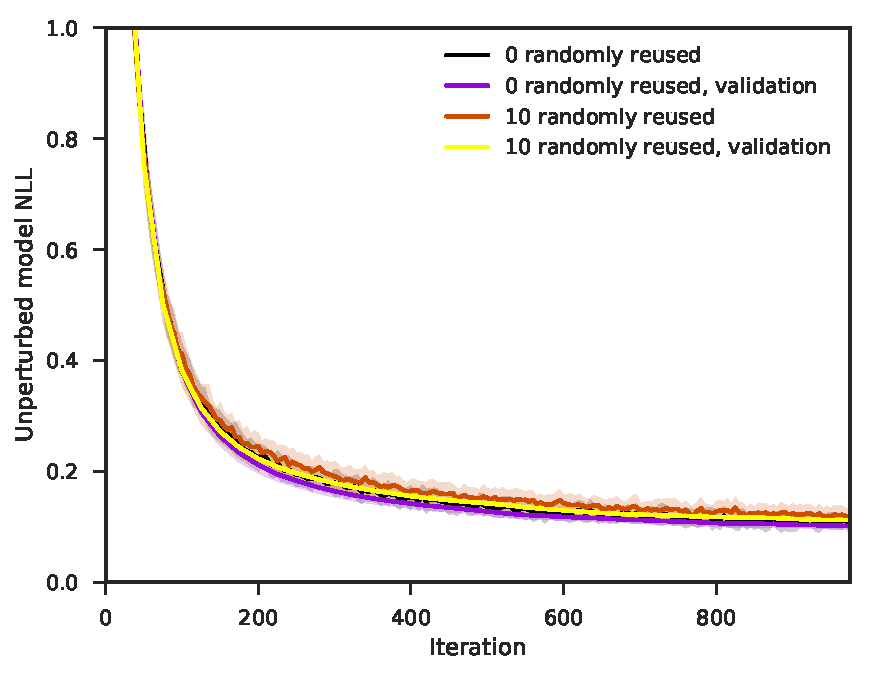
\includegraphics[height=5.8cm]{graphics/E026-IS-analysis/return_unp-all-series-mean-sd.pdf}
        \caption{}
        \label{fig: Theory: E026-IS-analysis/return_unp-all-series-mean-sd}
    \end{subfigure}
    \caption{
        Results of experiments with random resampling for the unperturbed model.
        \subref{fig: Theory: E026-IS-analysis/accuracy_unp-all-series-mean-sd} Training and validation set classification accuracy.
        \subref{fig: Theory: E026-IS-analysis/return_unp-all-series-mean-sd} Training and validation set \gls{NLL} loss.
    }
    \label{fig: Theory: E026-IS-analysis}
\end{figure}

One can note that randomly reusing perturbations is likely to break to assumption that the set of perturbations follows the search distribution, i.e. the Gaussian in this case. Since the gradient estimators rely on this assumption, the detrimental effect of random reuse of perturbations is expected. Importance mixing is designed to maintain the distribution of the perturbations but due to the collapse of the importance weights this is not the case in practice.






% \subsection{Adaptation sampling}
% \todo[inline]{Run the experiment on using adaptation sampling on \gls{MNIST} model}
% \todo[inline]{Discuss experimental results of adaptation sampling}





\subsection{Common random numbers}
This section presents results using the method of \gls{CRN}. The \gls{MNIST} network was trained using 100 perturbations with and without \gls{CRN} resulting in the training curves illustrated in \autoref{fig: Theory: E027-CRN-S-analysis}. \gls{CRN} was also tested in the \gls{RL} setting with resulting learning curves seen in \autoref{fig: Theory: E028-CRN-R-analysis}. The \gls{RL} runs were made using 40 perturbations for computational feasibility.

There is a small and almost insignificant benefit to using \gls{CRN} in the case of supervised learning on \gls{MNIST}. It can be seen that using \gls{CRN}, the training and validation accuracy and loss slightly outperform those of runs that did not use \gls{CRN} on average but within one standard deviation.

The method was also tested in the \gls{RL} setting with $45$ episodes simulated for each of the shared and random seeds versions.
The results are seen for Freeway in \autoref{fig: Theory: E028-CRN-R1-analysis/return_unp-all-series-mean-sd} and  Seaquest in \autoref{fig: Theory: E028-CRN-R2-analysis/return_unp-all-series-mean-sd}. The average population reward is plotted versus iteration number. 
The picture is similar to that of supervised learning with no significant improvement to be seen by using shared seeds for the simulations. 
As such, the method of \gls{CRN} cannot be concluded to improve on the \gls{VO} gradient estimate.

\begin{figure}[tbp!]
    \begin{subfigure}[b]{0.49\textwidth}
        \centering
        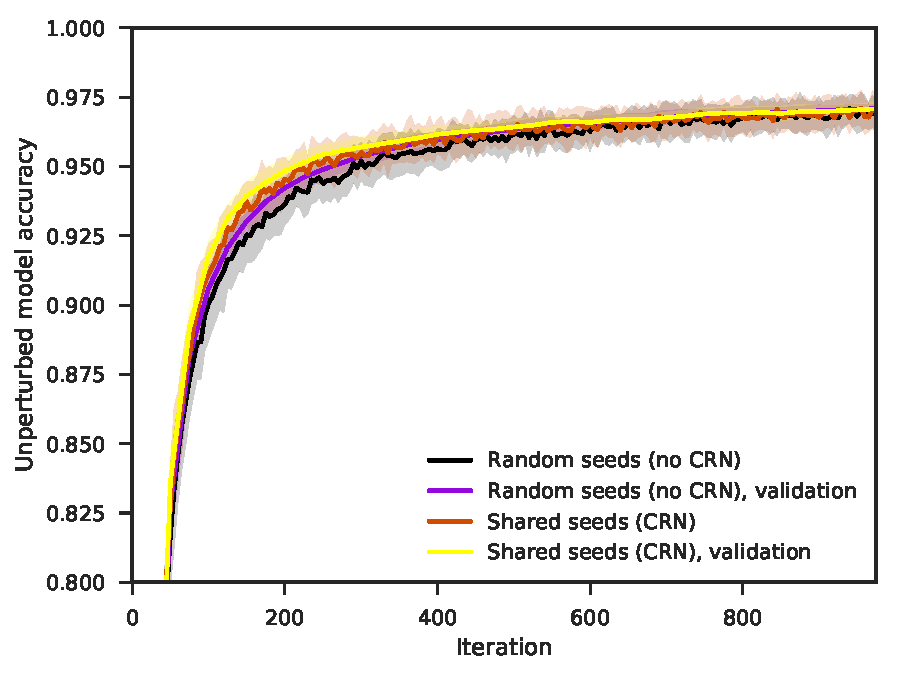
\includegraphics[height=5.7cm]{graphics/E027-CRN-S-analysis/accuracy_unp-all-series-mean-sd.pdf}
        \caption{}
        \label{fig: Theory: E027-CRN-S-analysis/accuracy_unp-all-series-mean-sd}
    \end{subfigure}
    \hfill
    \begin{subfigure}[b]{0.49\textwidth}
        \centering
        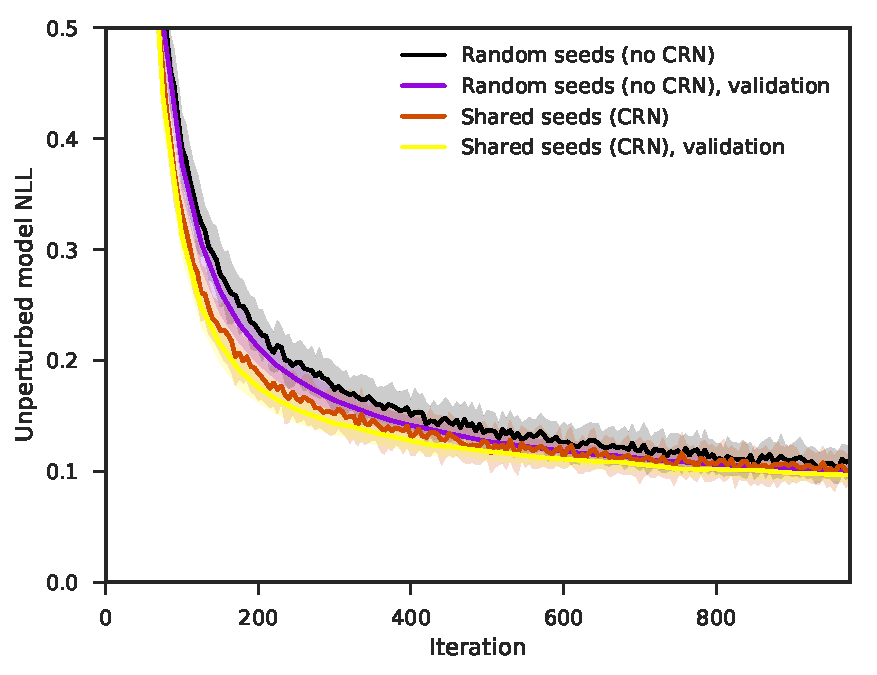
\includegraphics[height=5.7cm]{graphics/E027-CRN-S-analysis/return_unp-all-series-mean-sd.pdf}
        \caption{}
        \label{fig: Theory: E027-CRN-S-analysis/return_unp-all-series-mean-sd}
    \end{subfigure}
    \caption{
        Results of experiments with \glsfirst{CRN} for the unperturbed model run on \gls{MNIST}.
        \subref{fig: Theory: E027-CRN-S-analysis/accuracy_unp-all-series-mean-sd} Training and validation set classification accuracy.
        \subref{fig: Theory: E027-CRN-S-analysis/return_unp-all-series-mean-sd} Training and validation set \gls{NLL} loss.
    }
    \label{fig: Theory: E027-CRN-S-analysis}
\end{figure}
\begin{figure}[tbp!]
    \begin{subfigure}[b]{0.49\textwidth}
        \centering
        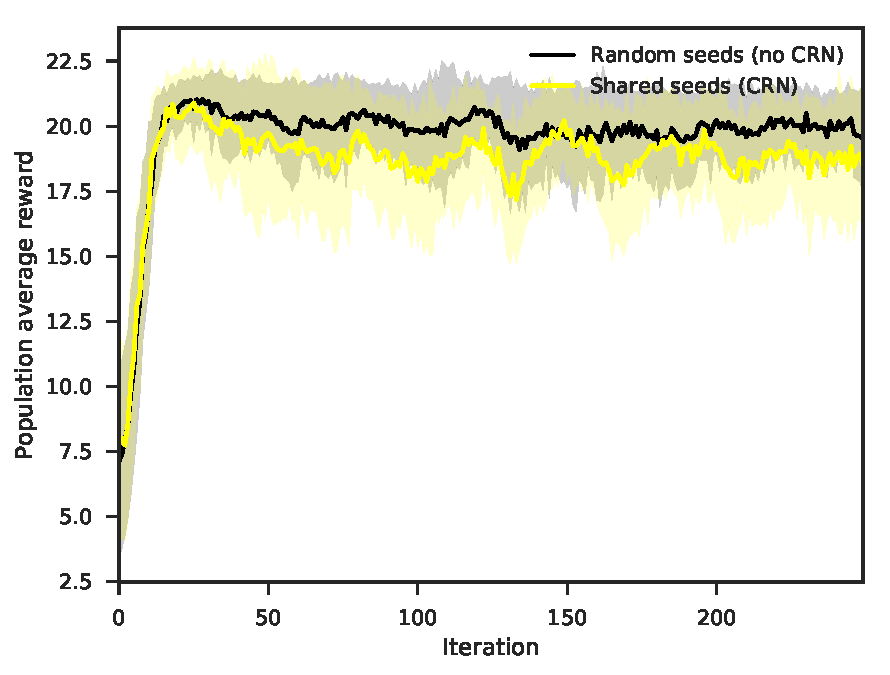
\includegraphics[height=5.8cm]{graphics/E028-CRN-R1-analysis/return_avg-all-series-mean-sd.pdf}
        \caption{}
        \label{fig: Theory: E028-CRN-R1-analysis/return_unp-all-series-mean-sd}
    \end{subfigure}
    \hfill
    \begin{subfigure}[b]{0.49\textwidth}
        \centering
        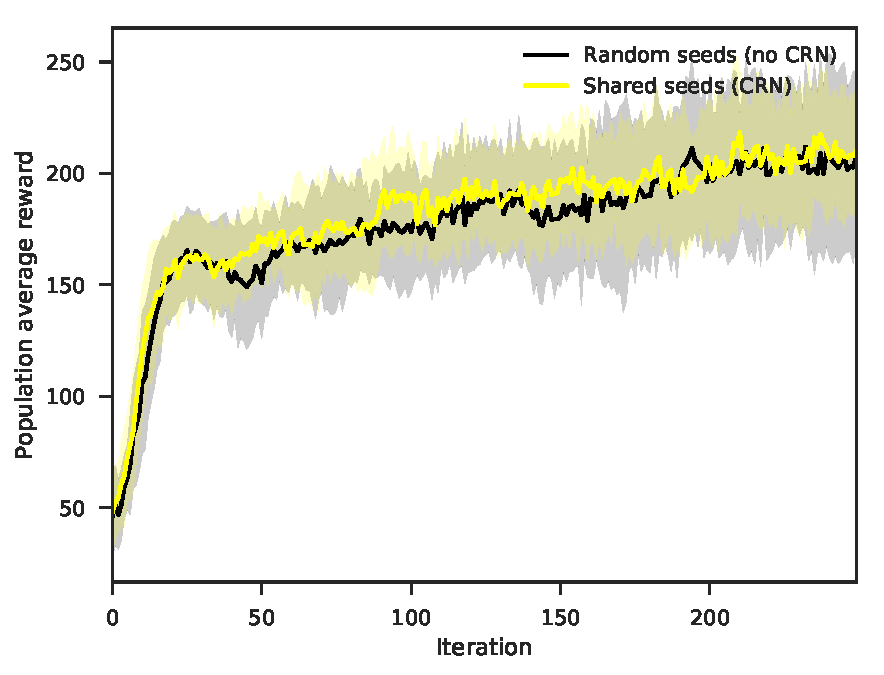
\includegraphics[height=5.8cm]{graphics/E028-CRN-R2-analysis/return_avg-all-series-mean-sd.pdf}
        \caption{}
        \label{fig: Theory: E028-CRN-R2-analysis/return_unp-all-series-mean-sd}
    \end{subfigure}
    \caption{
        Results of experiments with \glsfirst{CRN} for the population average on \subref{fig: Theory: E028-CRN-R1-analysis/return_unp-all-series-mean-sd} Freeway and \subref{fig: Theory: E028-CRN-R2-analysis/return_unp-all-series-mean-sd} Seaquest. The average reward of the population is plotted as a function of \gls{VO} iterations.
    }
    \label{fig: Theory: E028-CRN-R-analysis}
\end{figure}


